Para asegurar la reproducibilidad del análisis, todos los gráficos se generaron de forma automática con el script \texttt{plot\_generator.py}. Este script procesa directamente los datos crudos obtenidos por los algoritmos en C++ y guarda los archivos resultantes en la carpeta \texttt{code/implementation/data/plots/}.

\subsection{Análisis de Tiempo de Ejecución}

\begin{figure}[H]
    \centering
    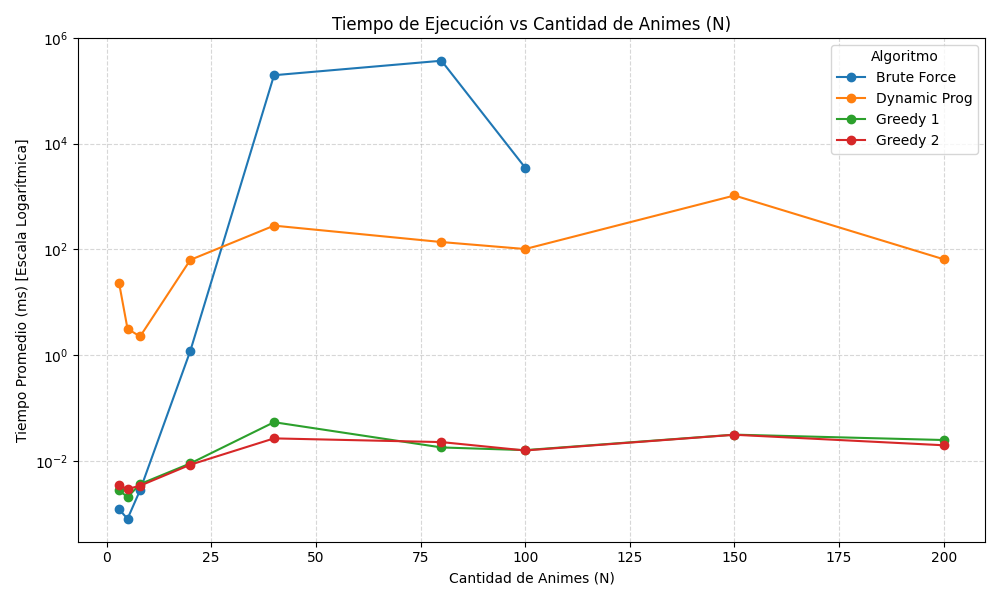
\includegraphics[width=0.8\textwidth]{../code/implementation/data/plots/tiempo_ejecucion.png}
    \caption{Tiempo de Ejecución promedio (en milisegundos) vs. Cantidad de Animes ($N$). Eje Y en escala logarítmica.}
    \label{fig:tiempo}
\end{figure}

En la \Cref{fig:tiempo} se puede ver el contraste tan marcado en los tiempos de ejecución de los algoritmos. Lo más relevante es lo que pasa con el algoritmo de Fuerza Bruta (línea azul), la ejecución se tuvo que cortar manualmente después de los casos con $N=100$. Para las instancias más grandes ($N \ge 150$), el tiempo para evaluar todo el árbol de decisiones creció tanto que superó la capacidad de procesamiento razonable del sistema, lo que causó que se cayera la terminal. 

Este corte en la gráfica no es considerable como un error en el script, sino la demostración en la práctica de su complejidad exponencial $O(31^N)$, lo que deja claro que este algoritmo es inviable para problemas grandes.

Por otro lado, la Programación Dinámica (línea naranja) completó todos los casos hasta $N=200$ en tiempos estables y polinomiales, mostrando variaciones que dependen más de los límites de recursos ($M$ y $E$) de cada archivo que del tamaño $N$ en sí. Finalmente, ambos algoritmos Greedy corren de forma lineal, con tiempos fraccionarios casi imperceptibles en la base del gráfico.

\subsection{Análisis de Uso de Memoria}

\begin{figure}[H]
    \centering
    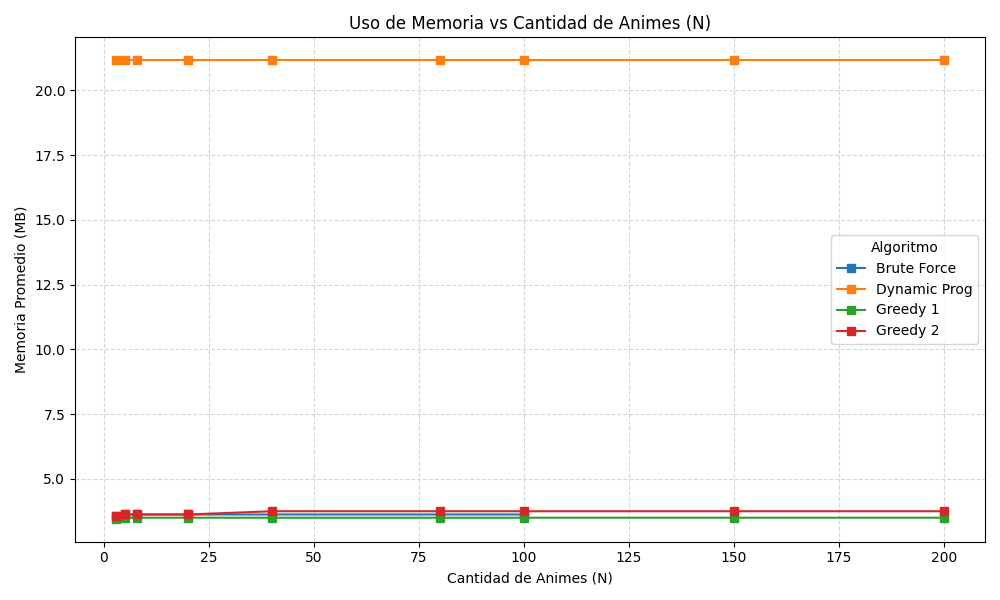
\includegraphics[width=0.8\textwidth]{../code/implementation/data/plots/uso_memoria.png}
    \caption{Consumo máximo de Memoria RAM (en MB) vs. Cantidad de Animes ($N$).}
    \label{fig:memoria}
\end{figure}

La \Cref{fig:memoria} muestra el uso de memoria que exige buscar una solución exacta. El algoritmo de Programación Dinámica mantiene un consumo de memoria plano y constante de $21.6$ MB, sin importar el número de animes $N$. Esto confirma exactamente lo esperado por la teoría: el espacio ocupado depende de las dimensiones fijas de la matriz de estados ($M=3000$ y $E=500$), dando una complejidad espacial de $O(M \times E)$.

En cambio, Fuerza Bruta y los Greedy muestran un uso de memoria bajísimo y constante (cercano a los $3.5$ MB), ya que solo necesitan almacenar las estructuras básicas del problema y la pila de llamadas de la recursión.

\subsection{Calidad de la Solución (Heurísticas vs. Óptimo)}

\begin{figure}[H]
    \centering
    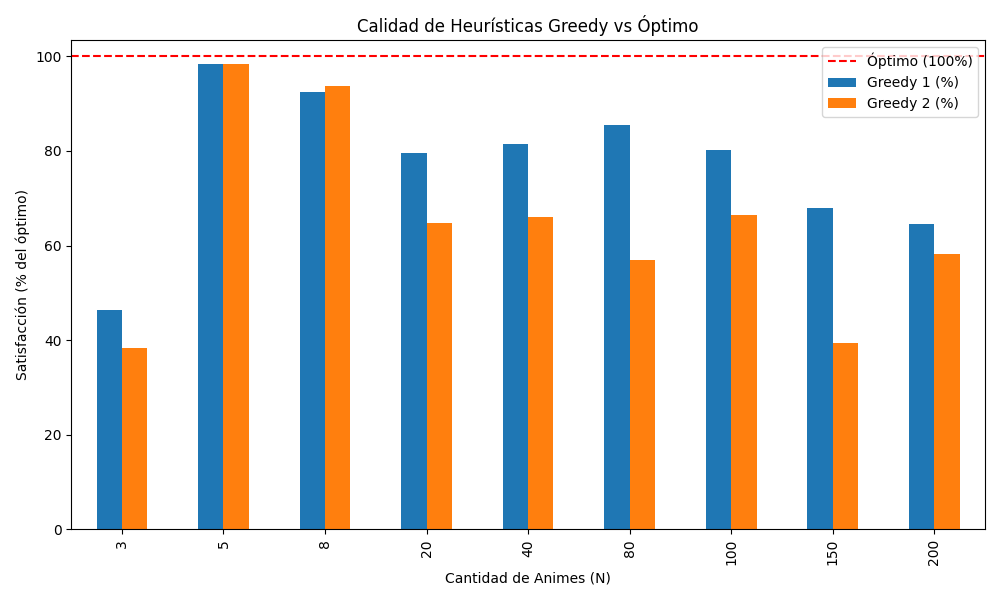
\includegraphics[width=0.8\textwidth]{../code/implementation/data/plots/calidad_solucion.png}
    \caption{Porcentaje de Satisfacción obtenido por las heurísticas Greedy en relación a la solución óptima}
    \label{fig:calidad}
\end{figure}

Como los algoritmos Greedy son muy rápidos pero no aseguran encontrar la solución óptima, la \Cref{fig:calidad} mide qué tan buenos son sus resultados comparados con el óptimo real que entrega la Programación Dinámica.

Se puede observar claramente que \textbf{Greedy 1} (que evalúa el ratio usando el costo combinado de tiempo y energía) supera por mucho a \textbf{Greedy 2} (que ignora la energía en el ordenamiento). Esto demuestra que, en problemas con restricciones múltiples, armar un criterio local que considere todas las variables del problema da como resultado soluciones subóptimas de mucha mejor calidad.